При тестировании классификатора использовались критерии оценки, описанные в разделе~\ref{eval}, 
а также время работы программы. Результаты работы классификатора представлены в таблице~\ref{tab:results}, а также
на рисунках~\ref{students_res:students_res}, \ref{google:google} и~\ref{github:github}.

\begin{table}[h!]
\caption{ Результаты работы }
\label{tab:results}
\begin{center}
\begin{tabularx}{\linewidth}{|X|X|X|X|X|X|}
\hline
\multicolumn{6}{|c|}{Набор данных <<Students>>} \\
\hline
Классифика- тор & Accuracy, \% & Precision & Recall & F1-score & Время работы, сек.\\
\hline
Random Forest & 89,55 & 0,90 & 0,93 & 0,90 & 93,61\\
\hline
AdaBoost & 70,45 & 0,70 & 0,74 & 0,70 & 53,22\\
\hline
ExtraTrees & 91,85 & 0,92 & 0,95 & 0,92 & 53,70 \\
\hline
\multicolumn{6}{|c|}{Набор данных <<Google Code Jam>>} \\
\hline
Классифика- тор & Accuracy, \% & Precision & Recall & F1-score & Время работы, сек.\\
\hline
Random Forest & 86,66 & 0,86 & 0,88 & 0,87 & 110,65\\
\hline
AdaBoost & 19,43 & 0,16 & 0,16 & 0,19 & 103,53\\
\hline
ExtraTrees & 88,09 & 0,88 & 0,90 & 0,88 & 60,34 \\
\hline
\multicolumn{6}{|c|}{Набор данных <<GitHub>>} \\
\hline
Классифика- тор & Accuracy, \% & Precision & Recall & F1-score & Время работы, сек.\\
\hline
Random Forest & 69,92 & 0,69 & 0,71 & 0,70 & 223,77\\
\hline
AdaBoost & 16,44 & 0,09 & 0,11 & 0,16 & 451,63\\
\hline
ExtraTrees & 70,99 & 0,70 & 0,72 & 0,71 & 201,13 \\
\hline
\end{tabularx}
\end{center}
\end{table}

\begin{figure}[h!]
\center{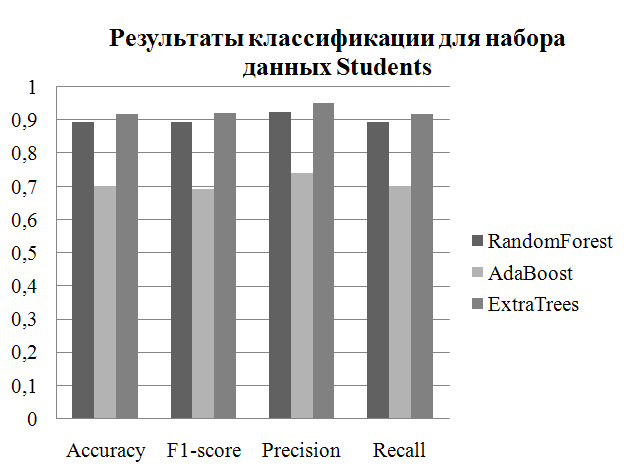
\includegraphics[width=0.6\linewidth]{students}}
\caption{ <<Students>> }
\label{students_res:students_res}
\end{figure}

\begin{figure}[h!]
\center{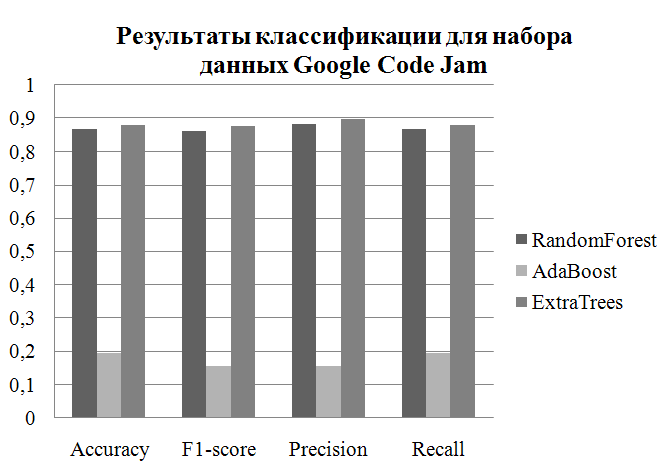
\includegraphics[width=0.6\linewidth]{google}}
\caption{ <<Google Code Jam>> }
\label{google:google}
\end{figure}

\begin{figure}[h!]
\center{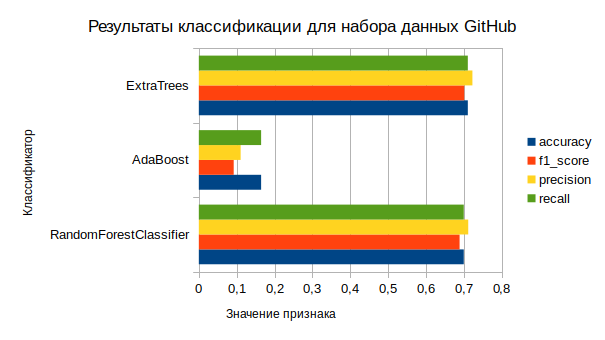
\includegraphics[width=0.6\linewidth]{github}}
\caption{ <<GitHub>> }
\label{github:github}
\end{figure}

Наихудшие результаты показал алгоритм AdaBoost, в то время как наиболее точным и быстрым из трех 
представленных алгоритмов оказался ExtraTrees (см. раздел~\ref{extra}). 

С использованием метода, основанного на извлечении лексических признаков и классификации с помощью алгоритма 
ExtraTrees (Extremly Randomized Trees) точность классификации составила 70-71\% на выборке данных из 30 авторов
и 2334 неполных, немопилируемых файлов с веб-хостинга GitHub. 

По результатам классификации можно сделать следующие выводы:
\begin{enumerate}
 \item заменив алгоритм классификации RandomForest
 на его модифицированную версию, ExtraTrees (Extremly Randomized Trees),
 можно повысить точность классификации, достигнутую в работе~\cite{git_blame},
 что в итоге, при воссоздании эксперимента коллег, даст наилучший результат классификации
 авторов исходного кода на языке С/С++ на сегодняшний день;
 \item исследованные методы могут применяться не только в <<лабораторных>> условиях, когда
тестовая выборка генерируется на основе студенческих работ или результатов олимпиад по программированию,
где решаются схожие задачи, ограниченные по времени и объему кода, но и в условиях реального мира.
\end{enumerate}


\clearpage